% -*- mode: fundamental -*-

% ****************************************************************

\chapter{BSV: FSMs}

\markboth{Ch \arabic{chapter}: BSV: FSMs}{\copyrightnotice}

\setcounter{page}{1}
% \renewcommand{\thepage}{\arabic{page}}
\renewcommand{\thepage}{\arabic{chapter}-\arabic{page}}

\label{ch_FSMs}

% ****************************************************************

\section{Introduction}

\index{BSV!FSMs}
\index{BSV!Finite State Machines}

So far, we have only been discussing pure combinational functions, for
which there is no concept of time.  Combinational functions are just
pure mathematical functions, ``instantaneously'' transforming input
values to output values.  However, a CPU, as shown in
Figure~\ref{Fig_FSMs_Simple_Instr_Exec}
\begin{figure}[htbp]
  \centerline{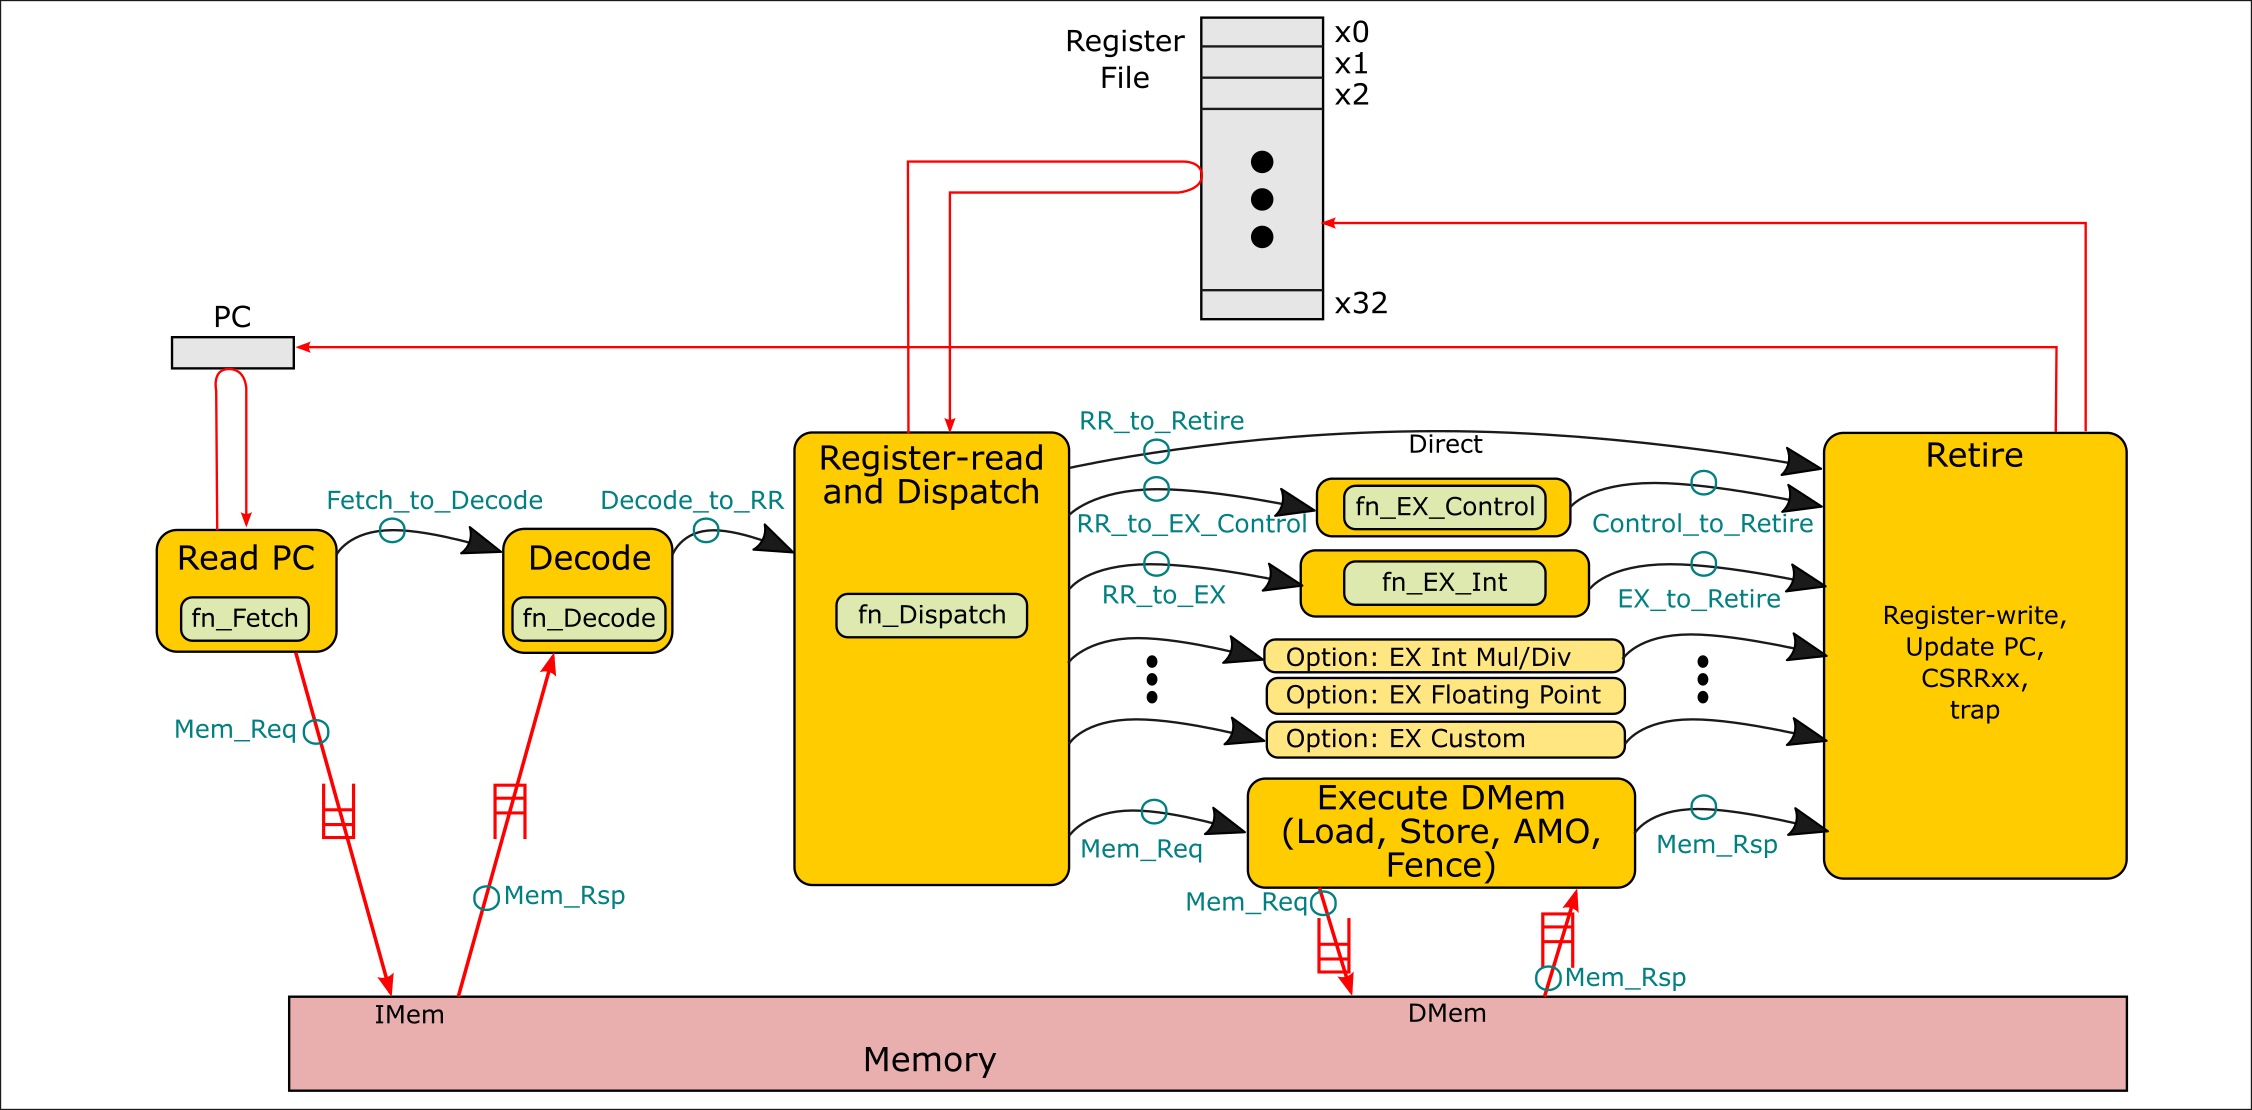
\includegraphics[width=6in,angle=0]{Figures/Fig_Instr_Exec_w_structs}}
  \caption{\label{Fig_FSMs_Simple_Instr_Exec}
           Simple interpretation of RISC-V instructions
	   (same as Fig.~\ref{Fig_Simple_Instr_Exec_w_structs})}
\end{figure}
represents a \emph{processs}, a behavior that evolves over time.  For
example the Drum CPU executes one full instruction after another,
repeating forever the flow along the black arrows in the diagram. For
each instruction, first it performs a Fetch operation, which sends a
request to memory. Some time later, the memory sends back a response,
which is then processed by the Decode step, Register-Read-and-Dispatch
step and then one of the Execute steps.  The Execute Memory Ops step
sends a request to memory. Some time later, the memory sends back a
response, which is processed in the Retire step.  Finally, it it loops
back to the Fetch step, and the process repeats for the next
instruction.

The simplest temporal process in hardware systems, perhaps the most
classical, is the \emph{FSM} (Finite State Machine).  A classical
notation for an FSM are so-called ``bubble-and-arrow'' diagrams: each
bubble represents a distinct \emph{state} of the system, and the
arrows connecting bubbles represent \emph{transitions} between states.
Transitions are typically enabled by some predicate condition on the
current state, and/or availability of some particular input from the
environment.  A transition moves the system to another state, and may
output something as well to the environment.  In bubble-and-arrow
diagrams, each arrow is often labeled with the condition that enables
the transition and any outputs produced by the transition.

\index{Drum!as an FSM}

Figure~\ref{Fig_FSMs_Simple_Instr_Exec} can be interpreted as a
bubble-and-arrow FSM diagram: each yellow rectangle (bubble) is a
state, and the process transitions from state to state, thereby
executing RISC-V instructions.  This is exactly what the Drum CPU
does.  Arros labels in our figure not conditions and actions, rather
the information (a struct) that is produced by one state and consumed
by another.

In this chapter we describe some special constructs for FSMs in BSV.
In the following chapters we will discuss using these constructs to
code the Drum CPU.

% ----------------
\vspace{2ex}

NOTE:
\fbox{\small
\begin{minipage}{5in}

In the literature one may read about FSMs where, from a state, we
could have a choice of transitions to different destination states.
These are called \emph{non-deterministic} FSMs.  In our designs we are
only concerned with deterministic FSMs where the conditions alway
identify a unique possible next state.

\end{minipage}}
% ----------------

% ================================================================

\subsection{Sequential FSMs, Concurrent FSMs, and Digital Hardware}

\index{BSV!FSMs!sequential {\vs.} concurrent}
\index{BSV!FSMs!concurrent {\vs.} sequential}

Classical FSMs in the literature are \emph{sequential} FSMs---every
transition is from the current state to a unique, particular next
state.\footnote{Even in non-deterministic FSMs, though there may be
several possible next-states, exactly one next-state is
non-deterministically chosen.}

Any digital system (including an entire computer) can theoretically be
viewed as a single (possibly giant!) FSM.  The current-state is the
current collective state of every register bit and every memory bit in
the system.  State transitions depend on the current state and any
external inputs.  Although theoretically correct, this is an
impractical, non-scalable, and not very useful way of viewing complex
digital systems.

Most non-trivial digital hardware systems are better viewed as
composed of multiple \emph{concurrent, communicating FSMs}, {\ie}
multiple classical FSMs running concurrently and independently and
communicating with each other (an output from one FSM may be an input
to another FSM).  Different BSV module instances are separate FSMs,
each running their own process(es).  These separate FSMs may
communicate with each other {\via} shared state (registers, fifos,
register files, {\etc}).  This is a more \emph{modular} and
\emph{scalable} way to think about complex digital systems.

\index{Drum!as a set of concurrent FSMs}

Even though Drum CPU execution is a sequential FSM, the overall system
can be viewed as a pair of concurrent FSMs: Drum and the Memory
System.  Each has its own internal FSM and behavior, and they
communicate memory requests and responses back and forth.

\index{Fife!as a set of concurrent FSMs}

For Fife, we will interpret \emph{each} yellow box in
Figure~\ref{Fig_FSMs_Simple_Instr_Exec} as its own FSM.  They all run
concurrently (and concurrently with the memory system), and
communicate various struct values (labels in
Figure~\ref{Fig_FSMs_Simple_Instr_Exec}) between the FSMs.

% ****************************************************************

\section{Rules and StmtFSM in BSV}

\label{Sec_Rules_StmtFSM}
\label{Sec_StmtFSM}

The fundamental behavioral/temporal primitive in BSV is the
\emph{rule} but we will postpone a detailed discussion of rules until
Chapter~\ref{ch_Rules_I}.  BSV's \verb|StmtFSM| is a higher-level
notation that captures the idea of certain \emph{structured}
processes.  \verb|StmtFSM| is ultimately implemented (by the
\emph{bsc} compiler) with rules, so it does not add any fundamental
semantic power to the language.

% ----------------
\vspace{2ex}

\begin{minipage}{1in}
HISTORICAL \\
NOTE:
\end{minipage}
\fbox{\small
\begin{minipage}{5in}

In a software program execution, the fundamental temporal ``flow''
primitive is from one instruction to the next, or a BRANCH or JUMP.
However, in most programming languages, we work at a much higher-level
of abstraction, using using such linguistic structures as
if-then-else, while-loops, for-loops, function calls and returns,
{\etc}.  Ultimately all these constructs are implemented (by a
compiler) in terms of the primitives, instruction
sequences/BRANCH/JUMP, and in that sense they do not add any
fundamental new semantic power to programming.  However, these
structured constructs are useful for humans: for readability, for
guiding our thinking, and for reasoning about the correctness of
programs.

\vspace{1ex}

Early programmers, {\eg} using first versions of the Fortran
programming language, worked directly with statement sequences (the
analog of instruction sequences) and ``GOTO'' statements (the analog
of BRANCH/JUMP), and their programs were a mess of control transfers
without any structure, sometimes called ``spaghetti code''.

\vspace{1ex}

In the 1960s, Edsgar Dijkstra, a Dutch computer scientist (later to
win the ACM Turing Award), recognized the importance of clear
\emph{structure} in composing programs.  In 1968 he wrote a famous
letter to the editor of the Communications of the ACM journal
(Association for Computing Machinery) titled ``Go To Statement
Considered Harmful'', a searing indictment of unstructured code.

\vspace{1ex}

The idea of constructing programs cleanly with nestable (composable)
structures (if-then-else, while-loops {\etc}), so called ``structured
programming'', grew out of that thinking; it is something we take for
granted today.

\end{minipage}}
% ----------------

\index{BSV!StmtFSM@{\tt StmtFSM}}

\verb|StmtFSM| is a sub-language within BSV for structured FSMs.  It
takes some basic, ``instantaneous'' actions, from which it builds
sequential processes that sequence these actions using conditionals
and loops.

We will use \verb|StmtFSM| to code Drum, which is a simple sequential
process.  It will not be adequate to code Fife, which is a collection
of concurrent FSMs; for that, we will use rules explicitly.

% ----------------
\vspace{2ex}

NOTE:
\fbox{\small
\begin{minipage}{5in}

We already briefly encountered a simple {\tt StmtFSM}, with just a
sequential block, in the testbench in
Section~\ref{BSV_small_testbench}.

\end{minipage}}
% ----------------

% ****************************************************************

\section{Actions and the {\tt Action} type}

\index{BSV!Action@{\tt Action}: primitive type of actions}
\index{BSV!actions}

The fundamental building-block for \verb|StmtFSM| is the ``action'',
which is a statement/expression of type \verb|Action|.  Some common
examples:

{\small
\begin{Verbatim}[frame=single, numbers=left]
   rg_pc <= rg_pc + 4;            // Assignment to a register
   f_Fetch_to_Decode.deq;         // Dequeue a fifo
   f_Decode_to_RR.enq (v);        // Enqueue into a fifo
   $display ("Hello, World!");    // Print something (in simulation only)
\end{Verbatim}
}

We discussed the \verb|Action| (and \verb|ActionValue|) types in
Section~\ref{Sec_Pure_vs_Side_Effect_functions}.  We used them in the
return type of the \verb|fn_Fetch| function in
Section~\ref{Sec_fn_Fetch}.  To recap, an expression with
\verb|Action| or \verb|ActionValue| type is one that potentially has a
side effect, as in each of the above example statements.

As discussed in Section~\ref{Sec_Register_syntactic_shorthands} the
first assignment statement is syntactic shorthand for:

{\small
\begin{Verbatim}[frame=single, numbers=left]
   rg_pc._write (rg_pc._read + 4)
\end{Verbatim}
}

{\ie} it is an invocation of the register \verb|_write| method which,
as described in
Section~\ref{Sec_Register_interface} has type
\verb|Action|.  Similarly, as described in
Section~\ref{Sec_FIFOF_interface}, fifo \verb|enq|
and \verb|deq| methods have return-type \verb|Action|, so the
statements \verb|f_D_to_RR.enq (v)| and \verb|f_D_to_RR.enq (v)| have
type \verb|Action|.

\index{BSV!display@{\tt \$display} has {\tt Action} type}

\verb|$display()| is a built-in construct in BSV that also has type
\verb|Action|.

% ================================================================

\subsection{{\tt Action} blocks: composing actions into larger actions}

\index{action@{\tt action}-{\tt endaction} blocks}

The \verb|Action| type is recursive: it is either a primitive action
(like those described just above), or it is a collection of things of
type \verb|Action|, collected using an \verb|action| block (bracketed
by the BSV keywords \verb|action| and \verb|endaction|).  For example
the above primitive actions can be collected into a single entity
which itself has type \verb|Action|:

{\small
\begin{Verbatim}[frame=single, numbers=left]
   action
      rg_pc <= rg_pc + 4;          // Assignment to a register
      f_F_to_D.deq;                // Dequeue a fifo
      f_D_to_RR.enq (v);           // Enqueue into a fifo
      $display ("Hello, World!");  // Print something (in simulation only)
   endaction
\end{Verbatim}
}

Although the actions in an \verb|action| block must be written in some
textual order, \verb|action| \emph{blocks do not involve any
sequencing.}  There is no temporal ordering of the actions in an
\verb|action| block.  All the actions in an \verb|action| block
(either directly in the block or, recursively in a sub-block) occur
``instantly'' and ``simultaneously''.  In the example above, lines 2-5
could have been written in any order with no change in
meaning/behavior.

% ================================================================

\subsection{Binding names in {\tt Action} blocks}

\index{let@{\tt let}-bindings in {\tt Action} blocks}

It is often convenient to give a meaningful name to a sub-expression
in an {\tt Action} block.  For example:

{\small
\begin{Verbatim}[frame=single, numbers=left]
   action
      Bit #(XLEN) next_pc = rg_pc + 4;
      rg_pc <= next_pc;
      $display ("Next PC is %08h", next_pc);
   endaction
\end{Verbatim}
}

Here, we bind the identifier \verb|next_pc| in line 2, and then use it
in lines 3 and 4.  We can often replace the type in the binding with
the keyword {\tt let}, if the type is obvious from the context:

{\small
\begin{Verbatim}[frame=single, numbers=left]
   action
      let next_pc = rg_pc + 4;
      rg_pc <= next_pc;
      $display ("Next PC is %08h", next_pc);
   endaction
\end{Verbatim}
}

The \emph{scope} of the identifier, {\ie} the region of program text
where it is available for use, is just the {\tt Action} block (and
inside any syntactically nested construct).

A binding, per se, \emph{is not an action!}.  It is just a
convenience, giving a name to the value of the right-hand side
expression.

Bindings (whether with a type or with \verb|let|) impose some ordering
on statements in the block: a binding of an identifier must precede
any use of that identifier.  In the previous two examples, line 2 (the
binding) must precede lines 3 and 4 (the actions), but lines 3 and 4
could be written in the opposite order.

% ****************************************************************

\section{{\tt StmtFSM}: sequences of actions}

\index{BSV!StmtFSM@{\tt StmtFSM}!seq@{\tt seq .. endseq}: sequences of actions}

Our first construct that has temporal behavior is the
\verb|seq|-\verb|endseq| block.  Each item in the block is typically
an entity of type \emph|Action|, and they are performed sequentially,
one after another.

{\small
\begin{Verbatim}[frame=single, numbers=left]
      seq
         ... action 1 ...
         ... action 2 ...
         ...
         ... action n ...
      endseq
\end{Verbatim}
}

\index{BSV!FSMs!Stmt@{\tt Stmt}: type of argument to FSM module constructors}

The \verb|seq| block itself has type \verb|Stmt|.  The items in a
block can have type \verb|Action| or the type \verb|Stmt|, {\ie}
\verb|seq-endseq| blocks can be nested.

The testbench in Section~\ref{BSV_small_testbench} contains an example
of a \verb|seq| block.

% ****************************************************************

\section{{\tt StmtFSM}: conditionals (if-then-else)}

\index{BSV!StmtFSM@{\tt StmtFSM}!if@{\tt if-then-else}: process conditional}
\index{BSV!if-then-else: ordinary expression \emph{vs} {\tt StmtFSM} process}

Conditional process execution can be expressed with traditional
if-then-else notation:

{\small
\begin{Verbatim}[frame=single, numbers=left]
   if ... Bool expression ...
      ... expression of type Stmt ...
   else
      ... expression of type Stmt ...
\end{Verbatim}
}

As usual, if-then-elses can be be nested.

% ----------------
\vspace{2ex}

NOTE:
\fbox{\small
\begin{minipage}{5in}

In Section~\ref{BSV_Combo_Circuits_if_then_else} we described ordinary
BSV if-then-else expressions, which often represent hardware
multiplexers, where both arms are ``evaluated'' (the hardware exists
for both sides) and the multiplexer merely selects one of the two
outputs.

\vspace{1ex}

{\tt StmtFSM} uses the same notation, but here it represents a
\emph{process}, and only one of the two arms is executed (like
if-then-else in most software programming languages).

\vspace{1ex}

There is no ambiguity in these two uses of if-then-else notation---the
context always clearly distinguishes what we mean, because there is no
overlap between ordinary expressions and {\tt StmtFSM} constructions.

\end{minipage}}
% ----------------

% ****************************************************************

\section{{\tt StmtFSM}: while-loops}

\index{BSV!StmtFSM@{\tt StmtFSM}!while@{\tt while}-loop repetition}

Repetitive processes can be expressed with traditional while-loop notation:

{\small
\begin{Verbatim}[frame=single, numbers=left]
   while (... Bool expression ...)
      ... expression of type Stmt ...
\end{Verbatim}
}

% ****************************************************************

\section{{\tt StmtFSM}: pausing until some condition holds}

\index{BSV!StmtFSM@{\tt StmtFSM}!await@{\tt await}: pausing until some condition}

An action in a \verb|StmtFSM| can be the \verb|await(b)| action, which
simply waits until the boolean expression in its argument evaluates to
true:

{\small
\begin{Verbatim}[frame=single, numbers=left]
   await (... Bool expression ...);
\end{Verbatim}
}

Of course, the \verb|StmtFSM| itself cannot cause the value the
change, since it is paused, and cannot change any state that would
cause the expression to change its value.  The state-change thus has
to be effected by some other part of the BSV design (a concurrent
FSM), not this particular \verb|StmtFSM|.

% ****************************************************************

\section{{\tt StmtFSM}: {\tt mkAutoFSM}: a simple FSM module constructor}

\label{Sec_AutoFSM}

\index{BSV!StmtFSM@{\tt StmtFSM}!{\tt mkAutoFSM} module}
\index{BSV!mkAutoFSM@{\tt mkAutoFSM} module in {\tt StmtFSM} library package}

Creating an FSM using \verb|StmtFSM| in BSV is a two-step process:

\begin{tightlist}

 \item Define the desired FSM behavior as an entity of type
       \verb|Stmt|.  Think of this as a \emph{specification} of
       desired behavior.

 \item Instantiate a module that takes this specification and
       implements the behavior.

\end{tightlist}

There are several \verb|Stmt| $\longrightarrow$ module constructors
available in the BSV library.  In this book we use only one of them,
\verb|mkAutoFSM|:

{\small
\begin{Verbatim}[frame=single, numbers=left]
   mkAutoFSM (... argument expression of type Stmt ...);
\end{Verbatim}
}

This creates an FSM with the behavior specified by the \verb|Stmt|
argument.  The FSM starts running immediately as we come out of reset,
starting at the first statement, and terminates when we fall through
the last statement.  Of course, it may never terminate if it contains
an infinite {\tt while} loop.

Note: ``terminating'' the FSM in simulation means it executes a
\verb|$finish()| action which stops the complete simulation.  In
hardware (where there is no concept of \verb|$finish()|) the FSM
simply goes idle.\footnote{Technically, none of the rules implementing
the FSM can fire any more.}  There may be other FSMs and rules in the
design that continue running.

% ****************************************************************

\section{{\tt StmtFSM}: many more features}

\index{BSV!StmtFSM@{\tt StmtFSM}!{\tt for}-loop repetition}

Here we have covered all the features of \verb|StmtFSM| that we need
for coding Drum.  There are many additional features that we skip
here, such as for-loops and repeat-loops, fork-join parallel blocks,
different kinds of modules instantiating \verb|Stmt|s, predicated
modules, and more.  We refer the reader to the FSM chapter in the
\emph{bsc Libraries Reference Guide} \cite{bsc_libs_ref_guide}.

The type \verb|Stmt| is a first-class type in BSV.  You can write
functions that have arguments and results of type \verb|Stmt|.  For
example, you might write a function that takes a numeric argument and
returns a \verb|Stmt|; this function can be invoked more than once to
produce multiple \verb|Stmt|s that differ because of the parameter.
Each of these \verb|Stmt|s can in instantiated into its own FSM.  This
further emphasizes the view that \verb|Stmt| is a specification of an
FSM behavior that is then instantiated in a module to produce that
behavior.

% ****************************************************************
